\section{Bestimmung des Ziels der Aufmerksamkeit}
\label{calc_Position}
Um das Ziel der Aufmerksamkeit einer Person zu bestimmen, muss die reale Position ermittelt werden. Die Orientierung des Gesichtes und die Blickrichtung können als Verlauf einer Ursprungsgerade betrachtet werden, mit em Ursprung an der Position des Gesichtes im Raum.\\
Ist der Ursprung und die Gerade bekannt, so kann ermittelt werden, ob sie durch bestimmte Punkte im Raum verläuft. Ist dies der Fall, so wird dieser Punkt wahrscheinlich betrachtet und ist Ziel der Aufmerksamkeit.
\subsection{Bestimmung der Position \& Orientierung des Gesichts}
Zur Bestimmung der Translation und Orientierung des Gesichtes wird ein CLNF bzw. PDM eingesetzt. Dabei wurde es mit der Kameraabbildung von 3D-Landmarks eines normierten Kopfes in verschiedenen Ausrichtungen initialisiert. Das normierte Ergebnis kann mit den passenden Kameraparameter von der Aufnahme angepasst werden um die reale Position und Orientierung zu bestimmen.
\subsubsection{Abschätzen der Kameraparameter}
Sind keine Kameraparameter bekannt, so können diese anhand der Bildauflösung grob geschätzt werden. Bei der Schätzung der Brennweite für ein Bild mit einer Dimension $I_x\times I_y$ wird das Standardobjektiv mit einer Auflösung von $640 \times 480$ Pixel angenommen, somit ergebenen sich die Brennweiten $f_x$ und $f_y$ wie folgt:
\begin{align*}
f_x = 500\cdot \frac{I_x}{640}\\
f_y = 500\cdot \frac{I_y}{480}
\end{align*}
\subsubsection{Position \& Orientierung}
\label{OpenFace_Pos_Ori}
Zur Bestimmung der Kopfposition $P= \begin{pmatrix}
X_{avg} & Y_{avg} & Z_{avg}
\end{pmatrix}^t$ im Kamerakoordinaten wird die Größe, ein Skalierungsfaktor der normierten Kopfgröße $S_G$, im Bild verwendet.\\
Da bei der Abbildung von Welt- nach Bild-Koordinaten gilt: $x=f\cdot \frac{X}{Z}$ und $ y=f\cdot \frac{Y}{Z}$, kann die Tiefe wie folgt abgeschätzt werden.\\
Sei $P_1 = \begin{pmatrix}
X_1&Y_1&Z_1
\end{pmatrix}^t, P_2= \begin{pmatrix}
X_2&Y_2&Z_2
\end{pmatrix}$ die Beschreibung der Größe $G$ eines Kopfes mit:\\
\begin{align*}
a &= \frac{\sqrt{(X_1-X_2)^2+(Y_1+Y_2)^2}}{\frac{Z_1-Z_2}{2}} =\frac{G}{Z_{avg}}\\
S &= \frac{S_G}{G}\\
\Rightarrow a\cdot f &= f\cdot\frac{G}{Z_{avg}} = S_G\\
Z_{avg} &= \frac{f}{S_G}\cdot G = \frac{f}{S}\\
X_{avg} &= \frac{x \cdot Z_{avg}}{f}\\
Y_{avg} &= \frac{y \cdot Z_{avg}}{f}\\
\end{align*}
Dies beschreibt allerdings nur eine Annäherung an die tatsächliche Position, da die Distanz mit Hilfe einer Durchschnittlichen Kopfgröße geschätzt wird.\\
\cite{OpenFace}
\subsubsection{Bestimmung der Blickrichtung}
\label{OpenFace_Blickrichtung}
Für möglichst genaue Ergebnisse wird für die Augenpartie ein weiteres CNN eingesetzt das nur auf diesem Bildaufschnitt arbeitet und weitere 28 Landmarks bestimmt. Durch diese werden die Lider, Iris und Pupille dargestellt und für jedes Auge separat bestimmt.\\
Zur Bestimmung der Blickrichtung wird wie folgt vorgegangen: Zuerst wird der Strahl bestimmt der, ausgehend vom Zentrum der Kamera, durch das Zentrum der Pupille verläuft. Nun wir der Schnittpunkt zwischen diesem Strahl und einer Sphäre bestimmt, die das Auge repräsentiert. Anschließend wird ein Strahl bestimmt der vom Zentrum der Sphäre ausgehend durch den berechneten Schnittpunkt verläuft, dies ist die resultierende Blickrichtung.
\subsubsection{Zusammenhang von Bildposition \& Weltposition}
Als Ausgangspunkt werden die Ergebnisse des CNN verwendet um die Position zu bestimmen. Zur Bestimmung der Orientierung $R$ liefert auch das CNN ein Ergebnis $R_{CNN}$. Allerdings stimmt es nur im Zentrum des Bildes, da am Rand immer mehr die Orientierung der einzelnen Pixel mit berücksichtigt werden muss.\\
\begin{align*}
euler_x &= \tan^{-1}(\frac{\sqrt{X^2+Z^2}}{Z^2})\\
euler_y &= \tan^{-1}(\frac{\sqrt{Y^2+Z^2}}{Z^2})\\
R_{pos} &= R(euler_x,euler_y,0)&\text{Umwandlung zur Rotationsmatrix}\\
R &= R_{CNN}\cdot R{pos}
\end{align*}
Eine weitere Verbesserung kann erreicht werden, indem die gefunden 2D-Landmarks mit Hilfe des PDM in 3D zu überführen. Um anschließend die Überführung von 2D nach 3D-Koordinaten erneut zu bestimmen um die Orientierung und Position zu ermitteln. Auch bei diesem Verfahren muss die Pixelorientierung beachtete werden. Allerdings ist auch ein Tiefendbild nötig, da ansonsten die Fehler weiter verstärkt werden. Daher ist es in der aktuellen Anwendung nicht sinnvoll einsetzbar.
\subsection{Größe und Genauigkeit}
Um die Qualität auf verschiedenen Distanzen zu ermitteln, wurde der Datensatz Forests for Real Time 3D Face Analysis \cite{database_Face_Ori} verwendet, da für jedes Gesicht die Position und Orientierung bekannt ist.
Die durchschnittliche Distanz zwischen Kamera und Kopf beträgt ca $70cm$ bei einer Kopfbreite von 78 Pixel. Um die verschiedenen Distanzen zwischen Probanden und Kamera zu simulieren, wurden die Bilder mit dem angegebene Skalierungsfaktor (X-Achse) verkleinert und mit dem Original verglichen.\\
Da verschiedene Verfahren zur Bestimmung der Position und Orientierung zur Verfügung stehen, sollen diese miteinander verglichen werden. Zur Bestimmung wurde nur das RGB-Bild verwendet und nicht zusätzlich die Tiefeinaufnahme, da dies in der Anwendung auch nicht vorhanden sind.
\subsubsection{Position}
Zur Bestimmung der Position gibt es zwei Verfahren, die direkte mittels Brennweite und Skalierung oder die Überführungsmatrix von 3D zu 2D Landmarks.\\
Die Funktionen Pose Camera und Pose World (Oben in \autoref{img_X_Pos}) verwenden die einfache Bestimmung mittels Skalierung. Dargestellt sind nur die X-Werte, da die Y-Werte eine recht ähnliche Verteilung aufweisen.\\
Bei den Z-Werten ergibt sich ein etwas anderer Verlauf, bei dem allerdings sie Fehlerquote bei kleinen Bildern gut sichtbar wird, siehe \autoref{img_Z_Pos}.\\
Der schnelle Abfall der Genauigkeit ist an der selben Stelle (0.5) an der auch die Detektionsrate stark absinkt, siehe \autoref{OpenFace_skal}. Somit kann das Verfahren bis zu seiner Grenze eingesetzt werden und erst, wenn die Detektion schwierig wird steigt auch der Fehler.
\begin{figure}
	\centering
	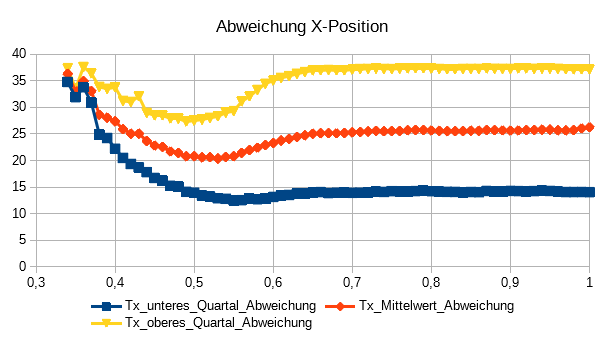
\includegraphics[width=0.45\linewidth]{tabelle/X_Pos_PC}
	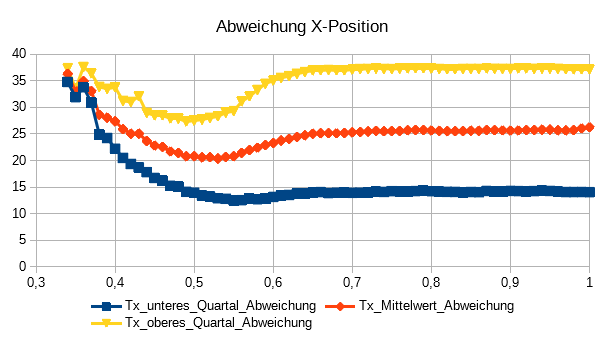
\includegraphics[width=0.45\linewidth]{tabelle/X_Pos_PW}
	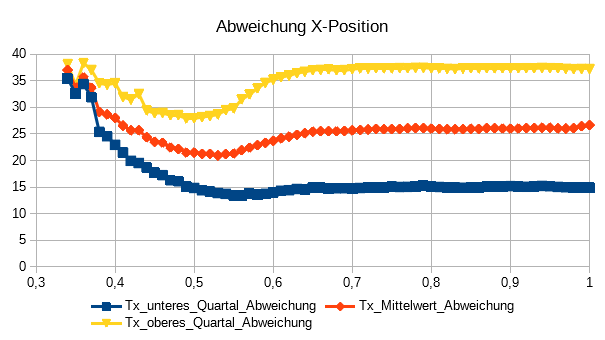
\includegraphics[width=0.45\linewidth]{tabelle/X_Pos_CPC}
	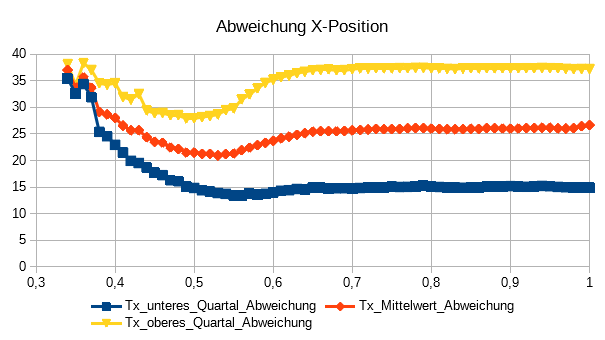
\includegraphics[width=0.45\linewidth]{tabelle/X_Pos_CPW}
	\caption{Pose World (links oben), Pose World (rechts oben), Correct Pose Camera (links unten) und Coorect Pose World, der Abstand (Y-Achse) ist in Millimeter.}
	\label{img_X_Pos}
\end{figure}
\begin{figure}
	\centering
	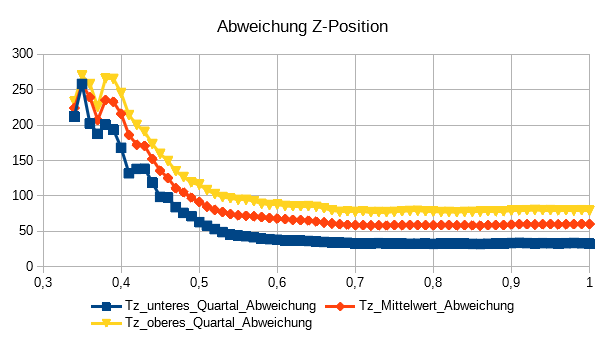
\includegraphics[width=0.45\linewidth]{tabelle/Z_Pos_PC}
	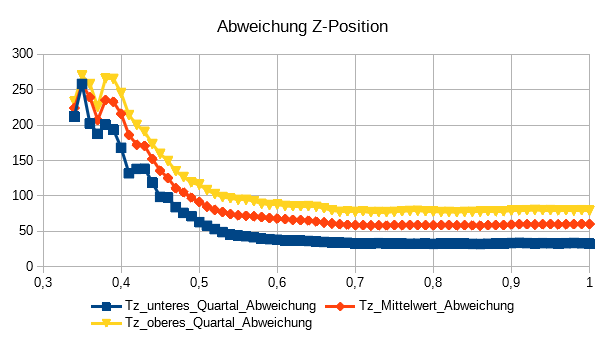
\includegraphics[width=0.45\linewidth]{tabelle/Z_Pos_PW}
	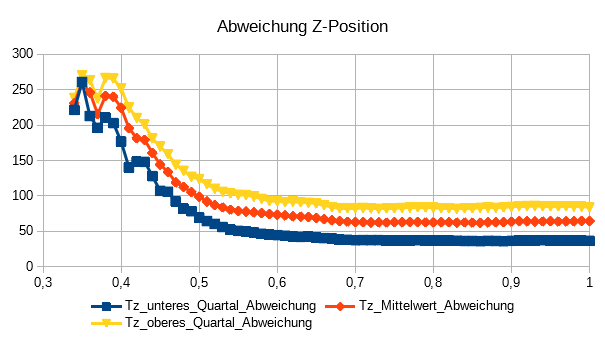
\includegraphics[width=0.45\linewidth]{tabelle/Z_Pos_CPC}
	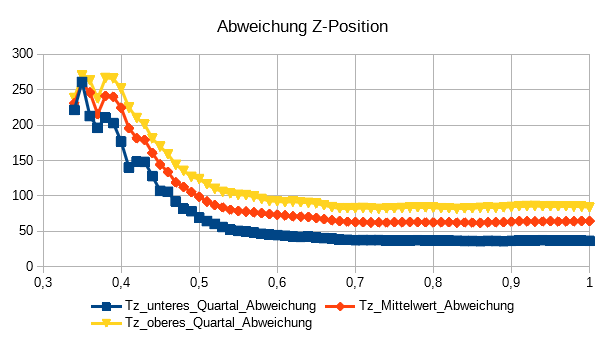
\includegraphics[width=0.45\linewidth]{tabelle/Z_Pos_CPW}
	\caption{Pose World (links oben), Pose World (rechts oben), Correct Pose Camera (links unten) und Coorect Pose World, der Abstand (Y-Achse) ist in Millimeter.}
	\label{img_Z_Pos}
\end{figure}
\subsubsection{Orientierung}
Auch bei der Orientierung werden die verscheiden Methoden miteinander verglichen. Die Analyse hat gezeigt, dass die Qualität der Verfahren von den einzelnen Rotationen abhängt.\\
Bei der X-Rotation, dargestellt in \autoref{img_X_Pot} können die rechten Verfahrenen (Pose World und Correct Pose World) überzeugen. Vor allem Pose World hat selbst bei kleinen Abbildungen nur eine mittlere Abweichung von $8.5^\circ$\\
Um die Y-Rotation zu ermitteln ist nun allerdings die linken (Pose Came und Correct Pose Came) den rechten (Pose World und Correcht Pose World) deutlich überlegen, siehe \autoref{img_Y_Pot}. Auch hier liegt der mittlere Fehler über lange Zeit bei etwa $9^\circ$.\\
Bei der Bestimmung von der Z-Rotation sind die Correct Pose Came und Pose Came nahe zu gleich gut, Correkt Pose World allerding schlechter und Pose World besser, siehe \autoref{img_Z_Pot}. Wobei auffällt, dass Pose World bei Werten unter 0.4 plötzlich der Fehler sehr stark zunimmt.
\begin{figure}
	\centering
	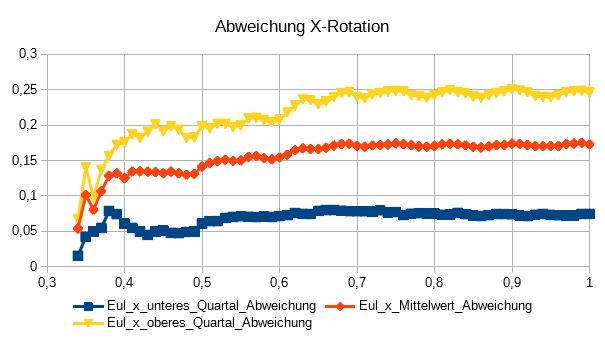
\includegraphics[width=0.45\linewidth]{tabelle/X_Rot_PC}
	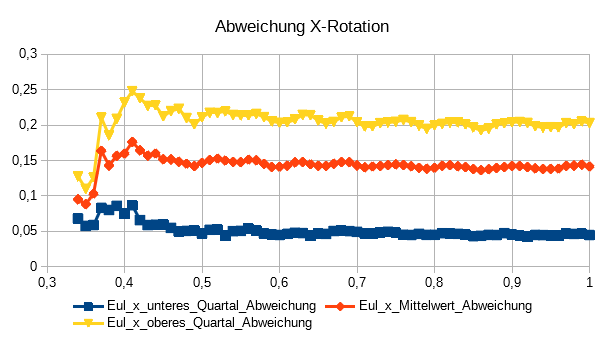
\includegraphics[width=0.45\linewidth]{tabelle/X_Rot_PW}
	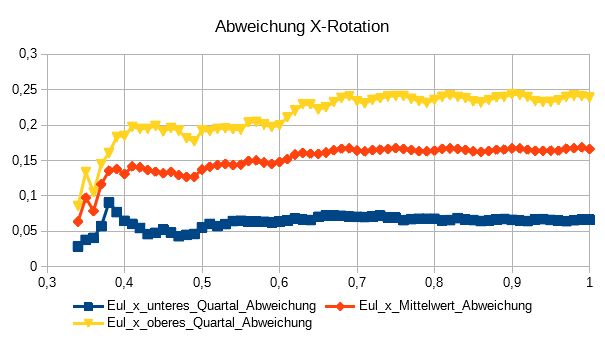
\includegraphics[width=0.45\linewidth]{tabelle/X_Rot_CPC}
	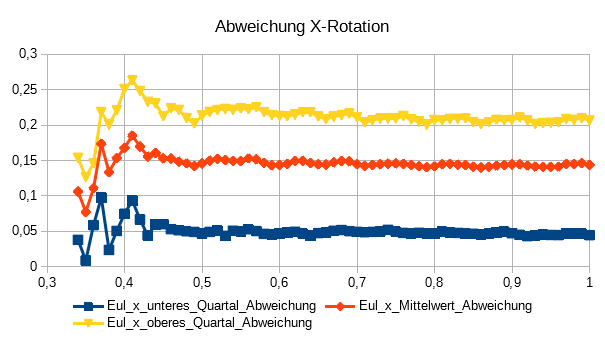
\includegraphics[width=0.45\linewidth]{tabelle/X_Rot_CPW}
	\caption{Pose World (links oben), Pose World (rechts oben), Correct Pose Camera (links unten) und Coorect Pose World, der Abstand (Y-Achse) ist im Bogenmaß.}
	\label{img_X_Pot}
\end{figure}
\begin{figure}
	\centering
	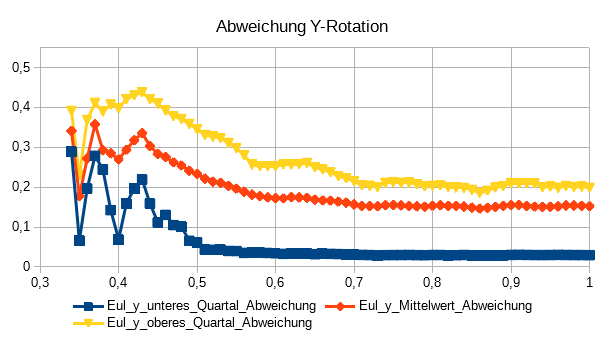
\includegraphics[width=0.45\linewidth]{tabelle/Y_Rot_PC}
	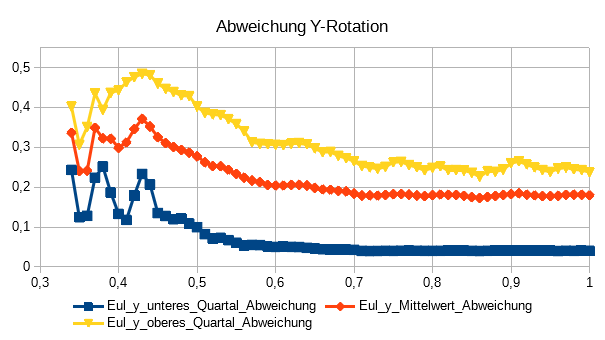
\includegraphics[width=0.45\linewidth]{tabelle/Y_Rot_PW}
	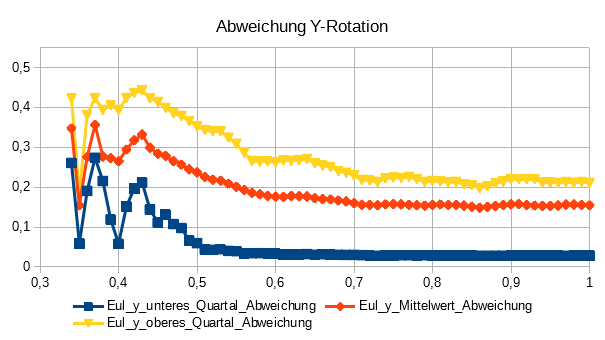
\includegraphics[width=0.45\linewidth]{tabelle/Y_Rot_CPC}
	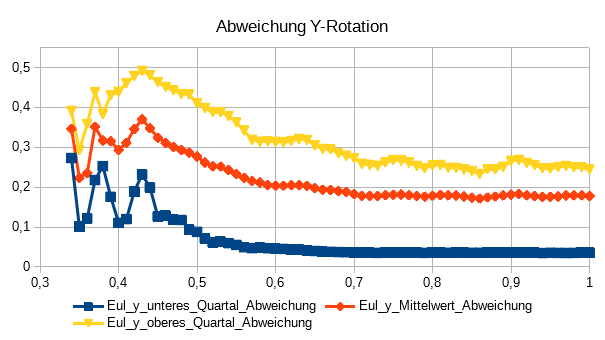
\includegraphics[width=0.45\linewidth]{tabelle/Y_Rot_CPW}
	\caption{Pose World (links oben), Pose World (rechts oben), Correct Pose Camera (links unten) und Coorect Pose World, der Abstand (Y-Achse) ist m Bogenmaß.}
	\label{img_Y_Pot}
\end{figure}
\begin{figure}
	\centering
	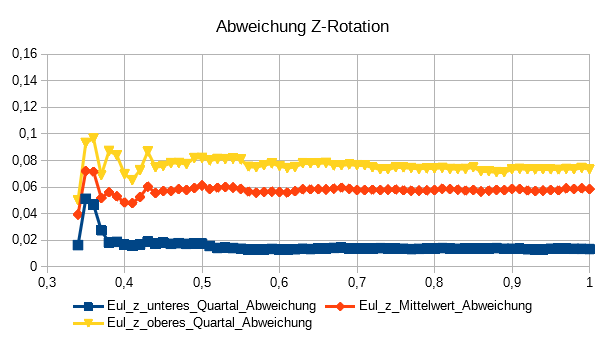
\includegraphics[width=0.45\linewidth]{tabelle/Z_Rot_PC}
	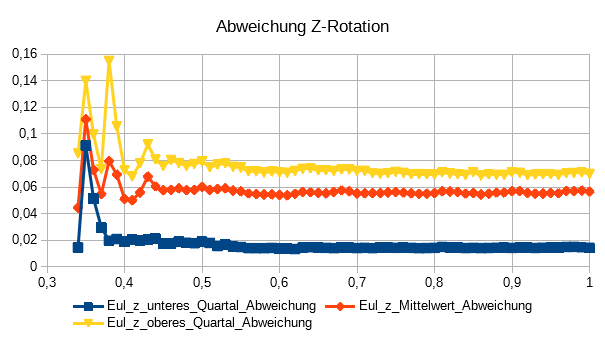
\includegraphics[width=0.45\linewidth]{tabelle/Z_Rot_PW}
	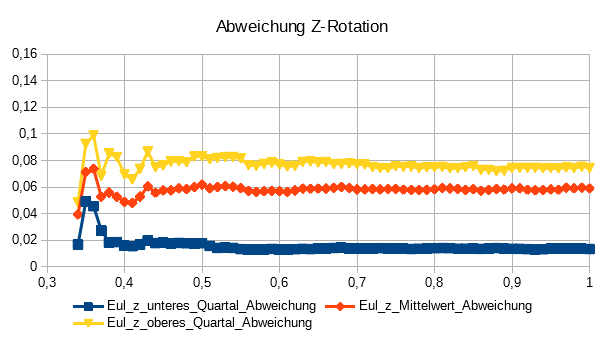
\includegraphics[width=0.45\linewidth]{tabelle/Z_Rot_CPC}
	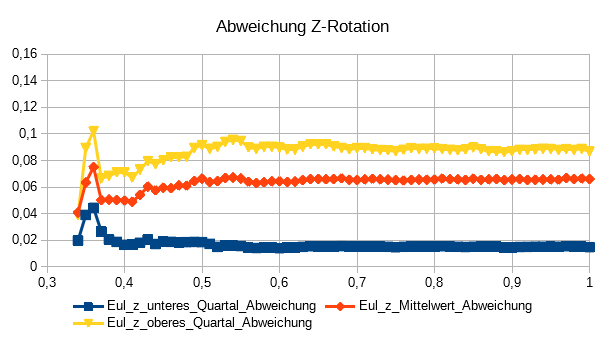
\includegraphics[width=0.45\linewidth]{tabelle/Z_Rot_CPW}
	\caption{Pose World (links oben), Pose World (rechts oben), Correct Pose Camera (links unten) und Coorect Pose World, der Abstand (Y-Achse) ist im Bogenmaß.}
	\label{img_Z_Pot}
\end{figure}
\subsubsection{Ergebnis}
Es zeigt sich, dass Pose World, also die einfache Bestimmung der Position mittels Skalierungsfaktor und zusätzlicher Korrektur der Wikel die besten Ergebnisse liefert.\\
Die Bestimmung mittels der Überführung von 3D zu 2D Punkten ist nicht notwendig, da ein schlechteres Ergebnis erzieht wurde.
\subsection{Bestimmung eines Punktes, auf der die Aufmerksamkeit liegt}
Von Interesse ist vor allem der Punkt auf den der Blick ruht bzw. das Gesicht ausgerichtet ist.\\
Bestimmung des Richtungsvektors $o$ aus der Rotationsmatrix
\[O= R\cdot (0,0,-1)^T\] 
Aus der Blickrichtung mehrerer Probanden kann auch der reale Punkt der Aufmerksamkeit ermittelt werden. Dazu wird die Blickrichtung als Linie $L_i = s \cdot n_i+ p_i$ beschrieben mit $s\in \mathbb{R}$ und $n_i,p_i \in \mathbb{R}^3$ verwendet.
\begin{align*}
c&=(\sum_{i} I -n_in_i^T)^{-1}
(\sum_{i} (I -n_in_i^T)\cdot p_i)
\end{align*}
Bei Verwendung der Gesichtsorientierung ergibt sich das Problem den konkreten Blickpunkt zu ermitteln, da die Augenbewegung nicht erfasst werden kann.
So muss ein Kegel, der den üblichen Bereich der Augenbewegung umfasst, um die Orientierung berücksichtigt werden als Fehlertoleranz und der gesamte Bereich kommt als Lösungen in Frage.
Außerdem liegt der Punkt der Aufmerksamkeit meist außerhalb des Bildbereiches der Kamera und muss entsprechend von einer Anwendung interpretiert werden.\\
Soll die Position des Ziels auf nahezu parallel verlaufende oder stark verrausche Ergebnisse berechnet werden, so ist die Bestimmung des Schnittpunkts nach dem obigen Verfahren nicht möglich.\\
Eine einfache Variante ist das Verwenden des durchschnittlichen Richtungsvektors $O_{avg}$ und Position $P_{avg}$ der Probanden. Die Tiefe $a$ muss nun geschätzt werden um das Ziel $P=O\cdot a$ zu bestimmen.